\section{Context}
\label{sec:context}
There are many localisation methods which could be used to create a navigation system for Bush House. However, many traditional localisation methods, such as GPS or GLONASS, are less accurate when used indoors. To better understand the localisation methods already available and the rationale for using Wi-Fi positioning, GPS \& GLONASS will be detailed in the following sections, along with alternative indoor positioning systems, and how they are relevant to the project scope.

\subsection{Global Positioning System and Global Navigation Satellite System}
\label{sec:gps-glonass}

The Global Positioning System (GPS\nomenclature{GPS}{Global Positioning System}) \cite{gps} is a space based navigation system developed by the United States. The system provides the geolocation information to a GPS receiver anywhere on Earth as long as its line of sight is unobstructed and as long as there are 4 visible satellites. GPS answers 5 questions: "Where am I?", "Where am I going?", "Where are you?", "What's the best way to get there? and "When will I get there?"\cite{gps}.

The Global Navigation Satellite System (GLONASS\nomenclature{GLONASS}{Global Navigation Satellite System}) is a similar navigation system, started by the Soviet Union and finished by Russia. GLONASS and GPS work in a similar way, but because of the smaller number of satellites for GLONASS, GPS is more accurate. Data from 2010 recorded by the Russian System of Differentional Correction and Monitoring show that the precision of GLONASS for latitude and longitude is 4.46–7.38 metres \cite{russian-monitoring-system}, whereas GPS-enabled smart-phones are typically accurate to within a 4.9m  radius under open sky \cite{gps-gov}. However, because of the positioning of the satellites, GLONASS is more accurate than GPS in the northern hemisphere. This is due to the fact that the development and positioning of satellites was started from Russia.

Nowadays, the manufacturers of GPS navigation systems say that adding GLONASS has made more satellites available to them, meaning that positioning works better than each of them individually when, for example, the line of sight for GPS is obstructed by buildings, and the microwaves will be weakened by walls or rooftops. Overall, a higher accuracy is achieved \cite{glonass-gps-1, glonass-gps-2} by using both of them combined. However, due to the fact that these two technologies need a direct line of sight in order to provide information about positioning, they suffer when used to determine the current location in indoors environments.

\subsection{Indoor positioning}
\label{sec:indoor-positioning}

As previously stated in section \ref{sec:gps-glonass}, GPS and GLONASS are not suitable for use indoors as the microwaves will be weakened by rooftops or walls
\cite{gps-indoor-precision}. To solve the issue, Indoor Positioning Systems (IPS\nomenclature{IPS}{Indoor Positioning System}) are used. IPSes are systems that can locate objects or people inside buildings using information collected by mobile devices \cite{ips-definition}. These systems can either be independent, or combined with GPS to achieve greater accuracy. IPSes use different technologies, such as Wi-Fi or Bluetooth enabled beacons \cite{ips-definition}. These technologies will be detailed in the following sections.

\subsubsection{Wi-Fi and Bluetooth based positioning}
\label{sec:wifi-positioning}

Most of the wireless technologies, such as Bluetooth beacons or Wi-Fia access points, can be used for detecting the location. In recent years, the Bluetooth technologies have been supported by many big companies, including Apple, mostly because of the recent developments in low energy Bluetooth sensors. The downside of Bluetooth beacons compared to Wi-Fi access points is that they don't provide an exact location, but rather a promixity composed of a geo-fence, rather than a pinned location. Moreover, in order to use Bluetooth beacons, dedicated Bluetooth devices need to be installed indoors, whereas most of the buildings already have a Wi-Fi infrastructure that provides Internet access. Considering this, a Wi-Fi navigation system can be built on top of the existing Wi-Fi access point systems available in Bush House.

\section{Methods used for Wi-Fi positioning}
\label{sec:methods-wifi-pos}
Having concluded that Wi-Fi positioning would be the most appropriate localisation method, in the following sections the different types of Wi-Fi positioning methods are considered for use in the navigation system and will be further explained.

% After opening access to Bush House, the floor plans of all the floors have been released. Using these, the positioning system works in two steps: 
% \begin{itemize}
%     \item Recording of locations in the building and mapping Wi-Fi measurements to them.
%     \item Positioning the user based on previously recorded data.
% \end{itemize}

% Recording is done by assigning values from the floor plan with measurements of the Wi-Fi signal measurements from the position recorded. By having as many positions recorded, the accuracy can be increased and localisation will work better.

% Localisation is done by measuring the signal strengths available currently and trying to find the location with the best match. This is done by calculating the location that has the smallest difference in signal strengths when compared to the data already recorded.

\subsection{Received Signal Strength Indication Localisation}
Received Signal Strength Indication (RSSI\nomenclature{RSSI}{Received Signal Strength Indication}) localisation measures the signal strengths from the available Wi-Fi access points around the device. It combines the information gathered, and finds out the distance from the device to the Wi-Fi access point. This method is usually combined with other methods of positioning, such as triliteration or triangulation in order to position the user, where the distance is measured using the signal's strength from the Wi-Fi access point.

\subsection{Fingerprinting Localisation}
\label{sec:fingerprinting-localisation}

Fingerprint localisation involves recording signal strengths from access points in different parts of the rooms, and then storing them into a database. This method is  RSSI based, because it records RSSI measurements taken around the building, but involves a more labour intense approach since the database needs to be kept updated in case the environment changes. Fingerprinting usually involves an offline phase, where positions are recorded in the database, and an online phase, where the data recorded is used to determine the location. In the offline phase, the signal strengths are measured at different fingerprints, or reference points. The location can then be calculated in the online phase  either in a deterministic way, by finding the closest match in the database, or by using a probabilistic model to see if the user may be in a certain position, using the data previously measured. One major drawback of this approach is that it requires for the database to be updated in case environmental changes happen, such as changing the position of furniture that will make some locations not accessible anymore. 

% The coordinates in latitude and longitude are used to determine the distance between two points and to determine the estimated time arrival between two points. When measuring, the mobile application has stored the corners of the building in latitude in longitude. Additionally, the corners of the device are measured in x and y coordinates and the 2D coordinates are attributed the latitude and longitude coordinates. By having this relation, for any 2D location on the floor plan, its location in latitude and longitude can be calculated, using the haversine formula. 

\subsection{Triliteration}
\label{sec:triliteration}

Another method used in combination with Wi-Fi positioning methods is triliteration. Triliteration is the process of determining locations using geometry shapes, such as circles and triangles. The location is calculated using two-dimensional geometry and three-dimensional geometry. Two-dimensional geometry is used by placing two circles to have a certain point lying on them, then the centres of the circles and the two radii provide sufficient information to reduce the possible locations to two. Furthermore, if a point lies on the surfaces of three spheres, then again, the centres of the spheres and the radii provide sufficient information to reduce the possible locations to two \cite{triliteration-methods}.

\begin{figure}[H]
    \centering
    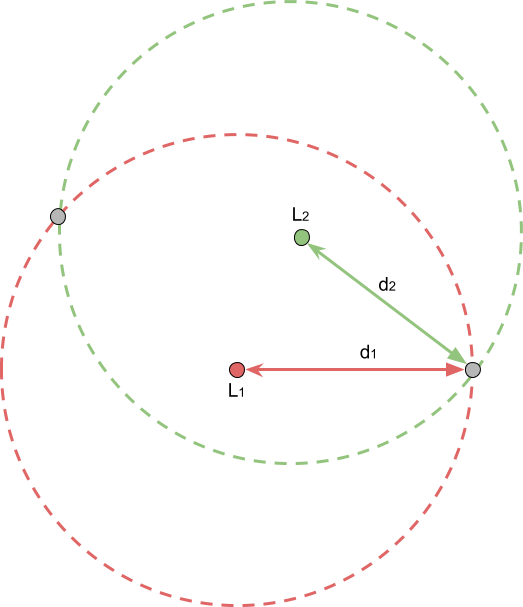
\includegraphics[width=170px, height=197px]{res/Trilateration2.png}
    \centering
    \caption{Triliteration with two circles \cite{triliteration-image}. $L_1$ and $L_2$ are the interest points, whereas $d_1$ and $d_2$ are the distances from those points to position $P$.}
    \label{fig:triliteration-2}
\end{figure}

Figure \ref{fig:triliteration-2} shows how triliteration first starts with two circles. The position P can be calculated by creating two circles that have the centres $L_1$ and $L_2$, with radii $d_1$ and $d_2$. The position can then be calculated using the radii and a set of equations. Using only two circles is not very accurate, since there are two possible results. In order to get the correct result, another circle can be added. By doing this, only one of the two possible results will be on the third circle, as seen in figure \ref{fig:triliteration-3}.

\begin{figure}[H]
    \centering
    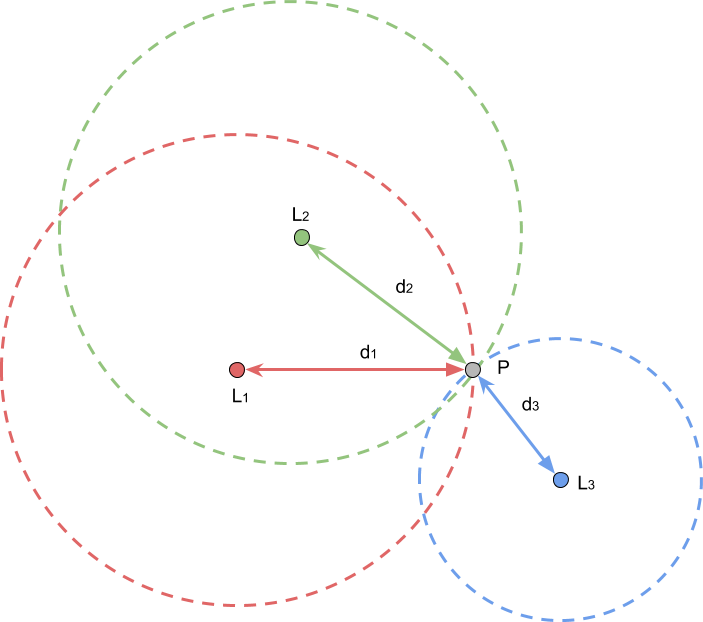
\includegraphics[width=170px, height=150px]{res/Trilateration3.png}
    \centering
    \caption{Triliteration with three circles \cite{triliteration-image}. $L_1$, $L_2$ and $L_3$ are the interest points, whereas $d_1$, $d_2$ and $d_3$ are the distances from those points to position $P$.}
    \label{fig:triliteration-3}
\end{figure}

% The above described methods for triliteration are used to calculate a point's latitude and longitude values, by knowing the corners' values in 2D points on the floor plan, and in latitude and longitude. The distances in the 2D plan can be easily translated into real life distances, using the already known coordinates of the corners. After this, the radii of the circles can be formed, and the intersection of the circles applied, finally finding the coordinates in latitude and longitude of the desired point. 

To conclude, the project's positioning algorithm will be an IPS that will use fingerprinting as the main method to collect location values, whilst the latitude and longitude will be calculated using triliteration.

\newpage
\section{Navigation}
After the position is determined, the user needs to find out how to get to other rooms. For this, locations registered on the floor plan, such as the rooms or any other destinations, can be translated into a graph structure. The locations can be seen as nodes, and the paths between them, as vertexes in the graph, where the cost is the distance between two locations, as seen in figure \ref{fig:graph}.

Building the graph gives way to use shortest path algorithms. For this project, Dijkstra's algorithm has been used, because this algorithm performs better when compared to a standard path finding algorithm, when there is little knowledge about the graph.

\begin{figure}[H]
    \centering
    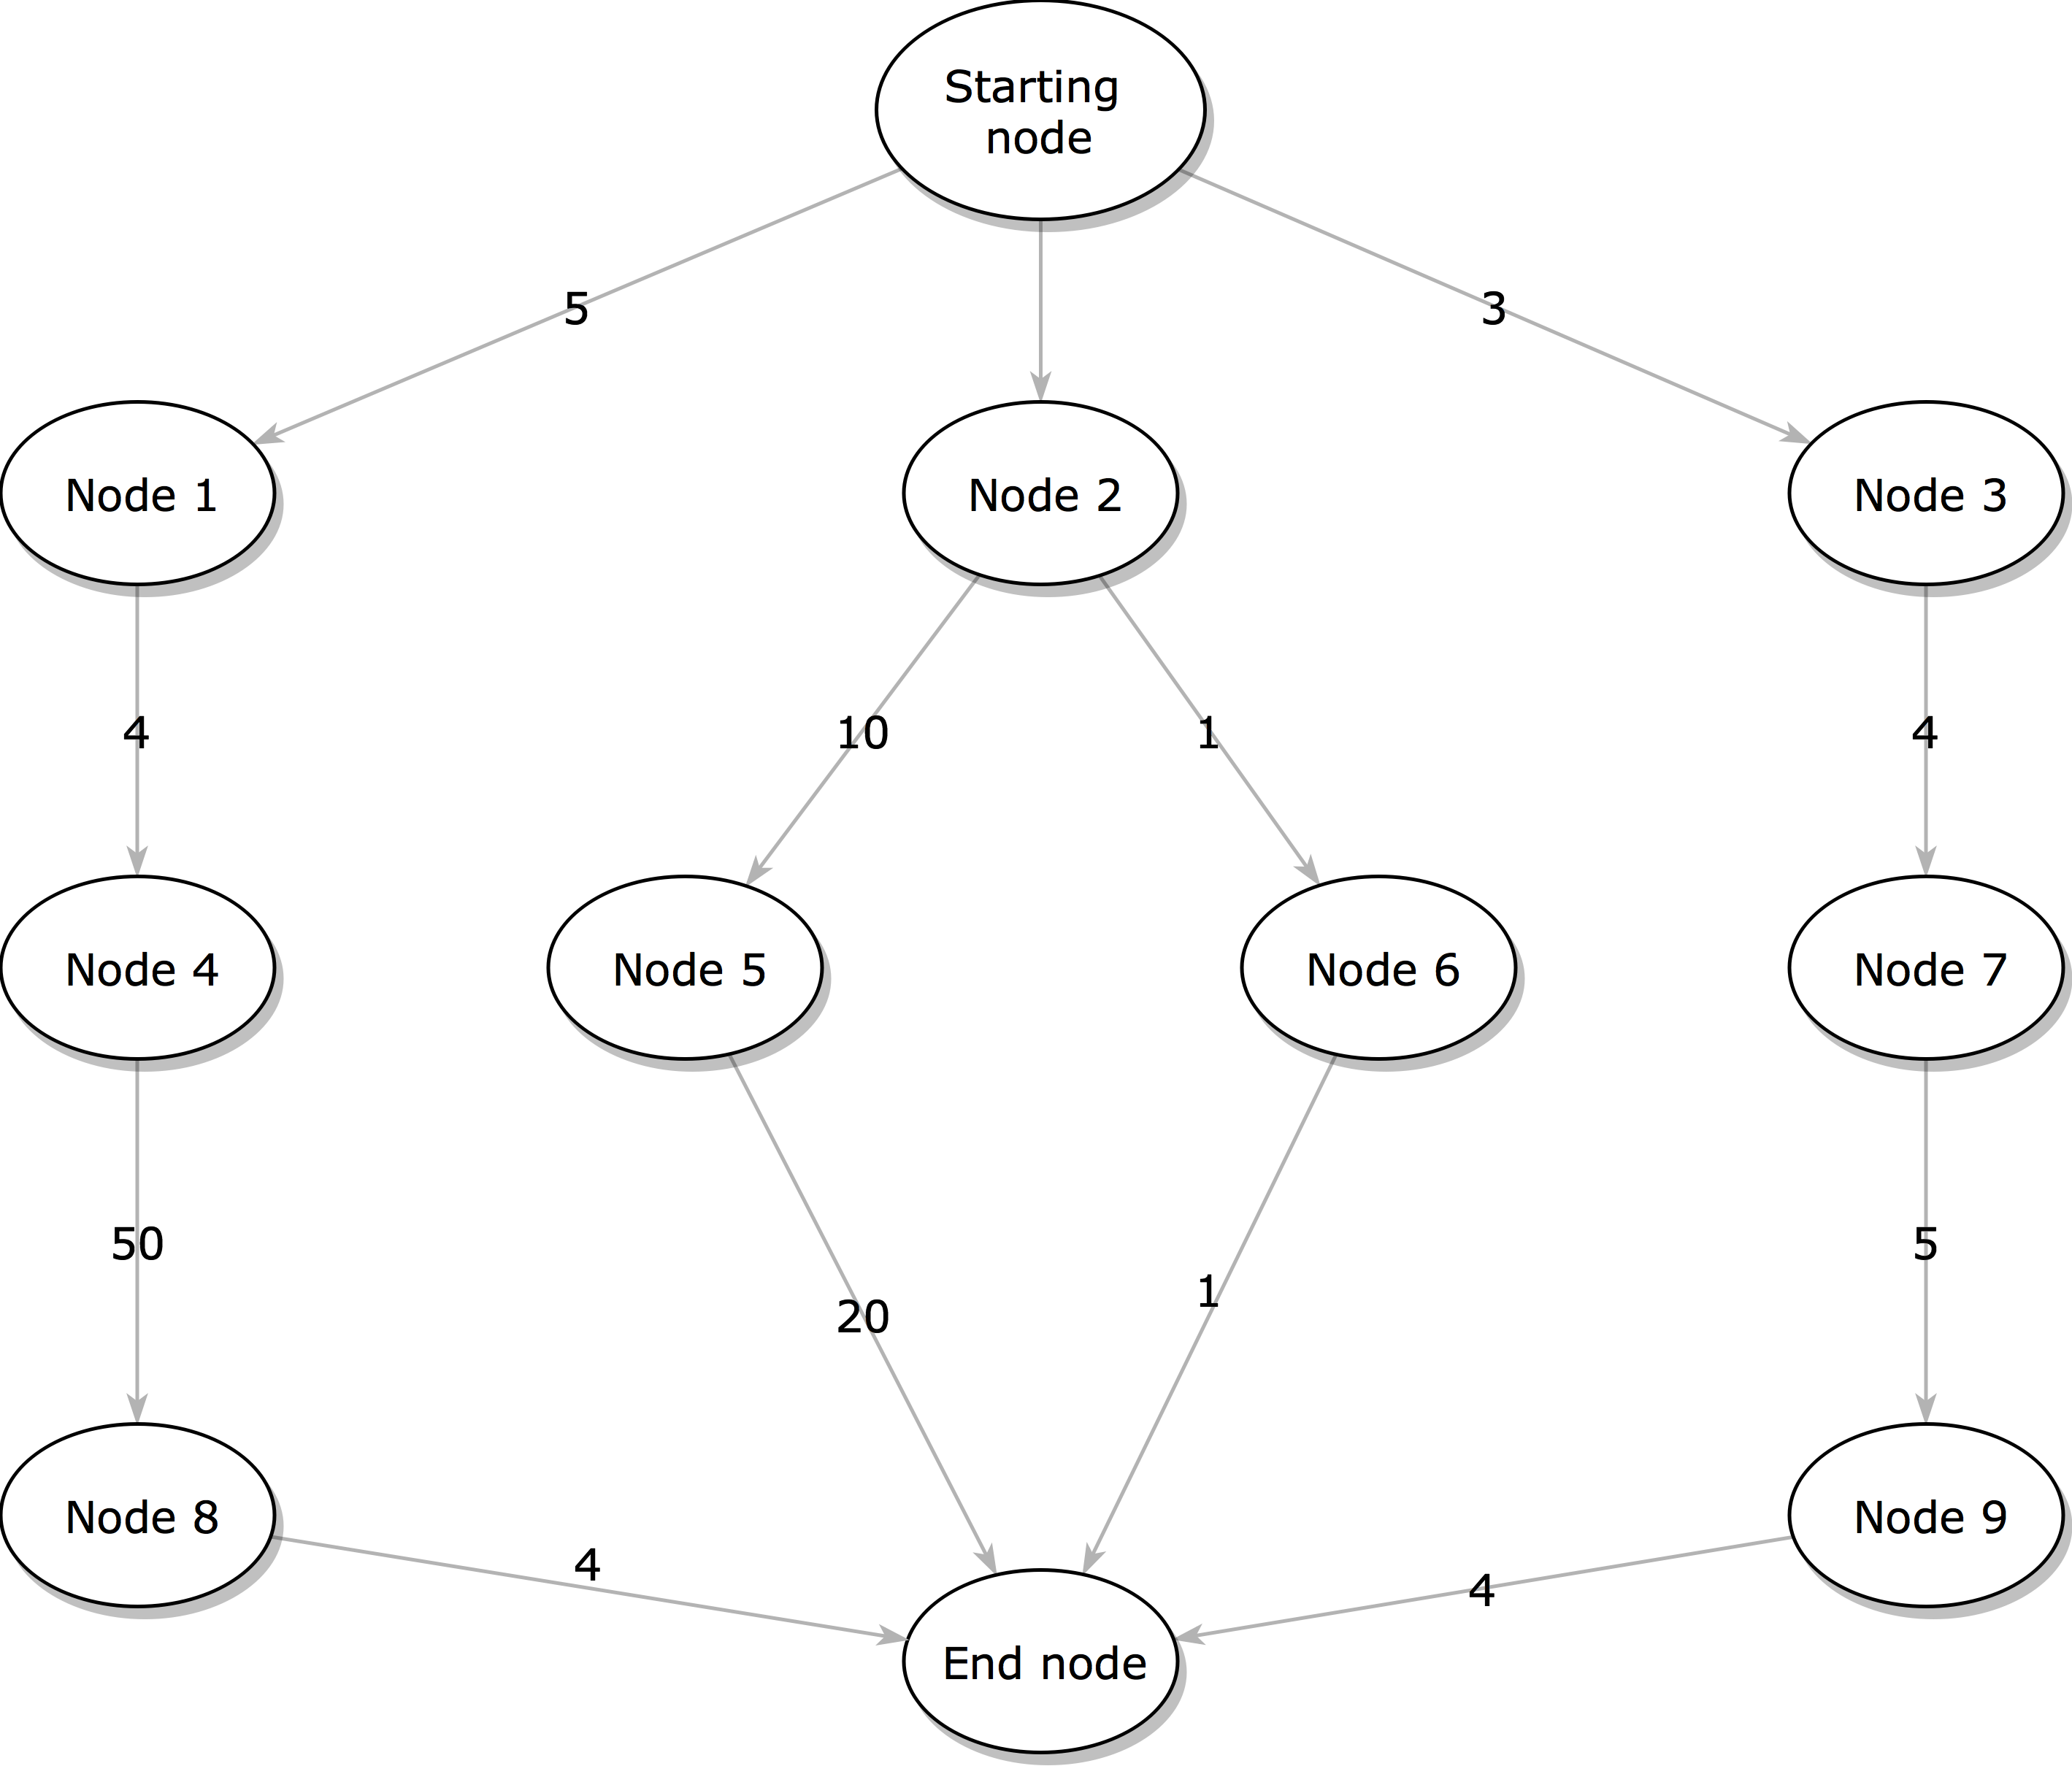
\includegraphics[width=235px, height=200px]{Background/graph.png}
    \centering
    \caption{A visual representation of a  graph. The circles represent the nodes, which are connected by lines, the vertexes. The numbers on each vertex represent the cost to get from a node to another node.}
    \label{fig:graph}
\end{figure}

\subsection{Haversine formula}
\label{sec:haversine}

\begin{align}
    a = sin^{2}(\frac{\Delta\phi}{2}) + cos(\phi_1) * cos(\phi_2) * sin^{2}(\frac{\Delta\lambda}{2})
\end{align}
\begin{align}
    c = 2 * atan2(\sqrt{a}, \sqrt{1-a})
\end{align}
    
\begin{align}
    d = R * c
\end{align}

The distance between nodes is calculated using the above formulae. Formula 2.1 is the haversine formula, in which the latitude ($\phi$) and longitude ($\lambda$) are used. The result is used in 2.2, in which $atan2$ is used. $atan2$ returns the value of the arc tangent of $\frac{y}{x}$ of two values $x$ and $y$, expressed in radians. Finally, the distance $d$ is calculated by multiplying the value computed in the 2.3 with $R$, the Earth's radius.

\subsection{Djikstra's Algorithm}
\label{sec:dijkstra}

Djikstra's algorithm is an algorithm that finds the shortest path between the nodes in a graph, either by building a shortest-path tree, that has a root in the source, or by calculating the shortest path between two points. Dijkstra's algorithm picks an the unvisited node from the graph with the lowest distance, calculates the distance through it to each unvisited neighbour, and updates the neighbour's distance if smaller. When the algorithm is done with neighbours, they are mark as visited, and they will be assigned the distance calculated.

\begin{figure}[H]
    \centering
    \fbox{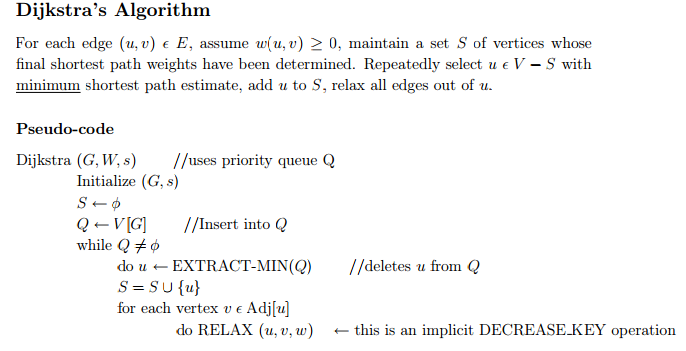
\includegraphics[width=400px, height=205px]{Background/dijkstra.png}}
    \centering
    \caption{Dijkstra's Algorithm \cite{cormen}. Describes the main Dijkstra algorithm used to find the shortest path between any two nodes in a graph.}
    \label{fig:dijkstra-algorithm}
\end{figure}

\begin{figure}[H]
    \centering
    \fbox{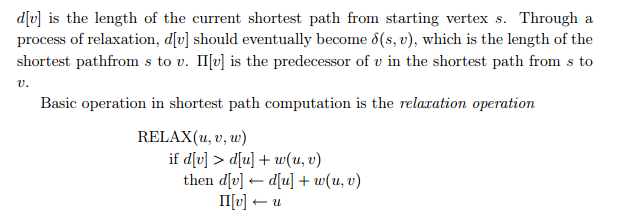
\includegraphics[width=400px, height=142px]{Background/relax.png}}
    \centering
    \caption{Relax procedure \cite{cormen}. This is used in the main Dijkstra algorithm from figure \ref{fig:dijkstra-algorithm} to get the shortest path.}
    \label{fig:relax-procedure}
\end{figure}

\section{Augmented Reality}
AR is defined as an enhanced version of the physical, real-world reality of which elements are added by computer-generated or extracted real-world sensory input such as sound, video or graphics \cite{ar-definition}. In other words, AR brings elements of the digital world into the user's perceived world, through either special devices, such as "Smart Glasses", or through a smart-phone's screen. The information shown is usually related to the local environment captured through the smart-phone's screen, and becomes interactive and digitally manipulable \cite{ar-definition-2}. The aim of AR in this project is to create a better experience for user, and a good example of this is to inform them about the timetable for the current week for a room that is near them.

\subsection{AR in Navigation}
% Combining AR with a navigation system can improve the effectiveness of the information shown. For example, car manufacturers have started showing information on the car's windshield, such as the final destination, current speed, speed limits or potential hazards in the paths \cite{ar-nav-1, ar-nav-2}. 

Combining AR with a navigation system can enhance the user experience and improve the effectiveness of the information shown. Because of this, many manufacturers have incorporated AR into their navigation systems. For example, in the car industry AR is used to show information such as the final destination, current speed, speed limits or potential hazards on the windshield.

A good example of how AR has improved navigation is NASA X-38 spacecraft. The spacecraft was flown using the LandForm software which overlaid map data on video to provide enhanced navigation for the spacecraft during test flights \cite{nasa-ar-nav}, such as taxiways, tower controls, or runways. This information has proved to be very useful in special conditions, such as low visibility. 

By following these examples, a similar solution will be developed in order to provide better navigation around Bush House. An arrow to follow will be shown on the screen when the user is navigating, and around the path, information about the rooms around will be shown. This information will include timetables and computers available in the computer labs positioned around the user.

\section{Related Work}

The subject of indoor navigation systems that use existing infrastructures of Wi-Fi connections has been researched into great detail. Many methods have been approached, including RSSI and fingerprinting.

% SpotFi \cite{spotfi} is a very good example of an algorithm that aims to build a very easy to use and deploy algorithm that also provides state of the art precision. The algorithm uses the angle of arrival of the Wi-Fi signal and the signal's time of flight. Using these two techniques, the algorithm has an error of 0.4m in most of the cases, and in more challenging conditions (such as only two Wi-Fi access points available), it has an error of 1.6m. Compared to other approaches, triliteration is not used to detect locations or paths.

% Wi-Fi positioning is explored by Evennou and Marx \cite{wifi-explore-paper}, where they try to improve the accuracy of the algorithm by using the smart-phone's sensors as well. The experiments start with a basic indoor mobile positioning that uses Wi-Fi which is progressively improved using a probabilistic model and a particle filter that removes errors. The algorithm takes into account maps of buildings that are available as bitmaps. Additionally, the paper shows how the a smart-phone's accelerometer and gyroscope can be used to improve the accuracy of positioning, by combining dead reckoning (accelerometer and gyroscope) with a Wi-Fi positioning system. The combination of the two greatly improves the trajectories. A simple triliteration approach, for example, produces a mean error of 5.73m, whereas if a particle filter and an INS are involved, then the mean error is reduce to 1.53m.

Active badges \cite{ips-survey-paper} was the first indoor positioning system, developed by AT\&T Cambridge. It involved an infrared sensor that was worn by a person. The locations in a building were covered with a network of infrared sensors. All the positions around the building of the fixed sensors were stored in an internal database, and the location of the badge could be then determined. In a similar way, AT\&T has developed an ultrasonic tracking technology \cite{ips-survey-paper}, that was supposed to be more accurate than the previous active badges. Users were tagged with ultrasonic tags, which emitted ultrasonic signals to receivers on the ceiling. Although it was accurate, the drawback of this was that it involved a large numbers of receivers to be mounted across the building; additionally, these receivers had to be placed and aligned, in order to provide accurate results \cite{ips-survey-paper}.

Shin, Cho and Cha have tried to automatically build an indoor map. Their algorithm, SmartSLAM \cite{wifi-map} is able to construct the indoor plan and draw the corridor outlines of the building. The approach taken by them uses fingerprinting and simultaneous localisation and mapping (SLAM\nomenclature{SLAM}{Simultaneous Localisation and Mapping}). SLAM is a localisation technique where a map of an unknown environment is constructed and updated while simultaneously keeping track of the current location within the map \cite{SLAM}. This approach is usually used for self driving cars, unmanned aerial vehicles, or even inside the human body \cite{SLAM-auto}. The system developed is the first one that uses SLAM on a smart-phone. However, Shin et al showed that this takes a toll on the battery, because the algorithm continuously scans the sensors which has a high energy use \cite{wifi-map}.

On the 29th of March, Apple has launched an application called "Indoor Survey App", that allows users to register buildings along with their floorplans in their system \cite{apple-indoor-survey}. Given these floorplans, then users are able to record locations by "dropping points" as "you indicate your position within the venue as you walk through". When registering these locations, the application uses a combination of Wi-Fi and radio signals to track positions; the application incorporates the solution used by WiFiSLAM, a company by Apple. This method provides a simpler and easier way to provide a data set to use for indoor positioning, by using already existing floor plans of the building. However, the only drawback of this is that locations need to be first recorded and kept updated by the admin users, in order to provide accurate results.

Another fingerprinting solution is COMPASS \cite{compass}. Positioning is achieved by registering reference points using the already existing Wi-Fi positions. Unlike a traditional fingerprinting approach, COMPASS adds the user's orientation received from the mobile phone's digital compass in order to improve the positioning. COMPASS has an accuracy of 1.65 meters, but it is important to mention that this is only an experimental approach that has not been tested on a large scale, but only in an environment of 312 square meters  \cite{compass}. Therefore, it is impossible to say how the system will behave on a much larger scale, outside the limits where it was tested \cite{compass}.

In conclusion, these papers and applications show that a very complex navigational system can be built on top of the existing sensors or Wi-Fi networks that are available, without requiring extra costs. Nowadays, most smart-phones are equipped with an accelerometer and a gyroscope. However, if a fingerprinting approach is taken, keeping a database with received signal strengths updated is very important. Future technologies will include methods that will try to reduce the time of building and managing this type of database \cite{wifi-explore-paper}.
